% Drawing 142/03-5 -- folder 142, batch 03, archive page 60 (PDF page 61).
% Transcription: une sphère : $P_\varepsilon \simeq P_{+}$ au sommet, $P_{\varepsilon'}$ en bas ; le quadrilatère $\widetilde{D}_r$ hachuré entre le méridien de $Q_i \simeq Q_\infty$ et celui du trou $R_{\omega i} \simeq R_1$ ; autour des trous les points $R_{\omega i}^{\omega}$, $S_i^{\varepsilon} \simeq S_0^{\varepsilon}$, $Q_{\omega' i}$ ; légende $r = (i, \omega, \varepsilon)$, $J = \ldots$
% Kind: sphere with a hatched quadrilateral. Method 2 (schematic redraw from the facsimile). Status: partial.
% Notes: Crop widened to the right to take in the legend. Pencil outline; P_epsilon = P_+ at the top, P_epsilon' at the bottom. From P_epsilon: the outer meridian down to Q_{omega' i} at the left edge, the meridian to S_i^epsilon = S_0^epsilon at the top of the left hole, the thick vertical arrow to Q_i = Q_infty, and the meridian to S^epsilon_{omega' i} at the top of the right hole; the quadrilateral tilde D_r between the second meridian and the arrow hatched in pencil. The equator in front from Q_{omega' i} round the left hole (its small circle) through Q_i to the right hole (its small circle), the back of the equator in pencil; from the bottom of the left hole and from Q_i the two meridians down to P_epsilon'. Every stroke ends at the same vertex points. Labels round the holes as read: R^omega_{omega i} on both sides of the left hole with simeq R_1 under the right one, S_i^{epsilon'} under it; R^{omega'}_{omega i} and simeq R_1^- at the right hole, R_{omega i} simeq R_1 at its centre. Legend r = (i, omega, epsilon), J = at the right. Nothing is struck. Redrawn 2026-11-09 (issue 128); overlay check 2026-11-13 (issue 147). Second pass 2026-11-14 (issue 147, Claude claude-opus-5-5): the pencil hatching of tilde D_r, drawn before as a regular pattern, is redrawn stroke by stroke from a contrast-enhanced 26 px/unit gridded crop of the 400 dpi colour scan: eleven faint parallel strokes rising to the right, not evenly spaced and of unequal length, and the two thin pencil strokes from P_epsilon that bound the hatching (one beside the thick arrow, one beside the meridian to S_i^epsilon). Rasterised by the session's previewer (not compiled: no TeX in the session) and laid over the crop: the hatching strokes lie on their ink to within about 1 unit. Still differs: the left hole is a blot and the labels round it are overinked (their indices are a reading); the label in the hatched region reads like tilde I_r with a stroke through it and is set tilde D_r as in the transcription; Q_{omega' i} is cut by the left edge of the crop. Not checked by a reader.
% Coordinates: 1 unit = 1 mm = 1/100 of the crop width (bbox in page fractions: [0.14, 0.27, 0.4, 0.45]).
% Redrawn by Claude (claude-opus-5-5), issue #73, 2026-11-09; not checked by a human; not compiled (no TeX in the session).
% Checked by Claude (claude-opus-5-5) 2026-11-13 (issue #147): overlaid on the 400 dpi colour facsimile; not compiled (no TeX in the session). Not checked by a human. Status: partial.
% Second pass by Claude (claude-opus-5-5) 2026-11-14 (issue #147): redrawn stroke by stroke from the 400 dpi colour facsimile, overlaid on a grid; not compiled (no TeX in the session). Status: partial.
% Rights: reproduces part of the work -- behind RENDER_TRANSCRIPTS, never published by itself.
\documentclass[tikz,border=3pt]{standalone}
\usepackage{amsmath,amssymb}
\usetikzlibrary{patterns,arrows.meta}
\tikzset{pencil/.style={black!45}, struck/.style={black!35}, mark/.style={circle,draw,inner sep=1.3pt}, pt/.style={circle,fill,inner sep=0.9pt}, opt/.style={circle,draw,fill=white,inner sep=1.1pt}}
\begin{document}
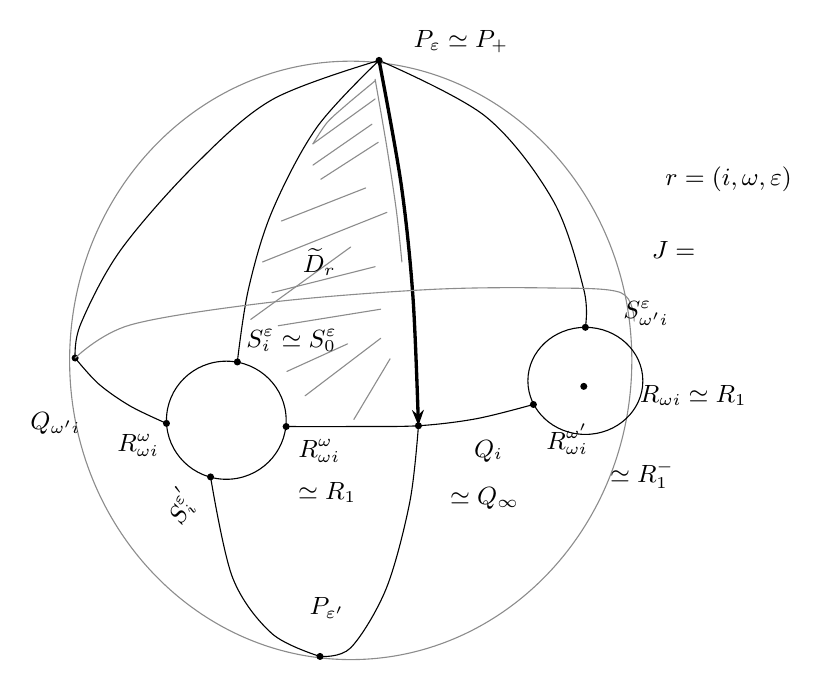
\begin{tikzpicture}[x=1mm,y=1mm,line cap=round,line join=round,font=\scriptsize]
\draw[pencil] (40,-51) ellipse[x radius=35.7, y radius=38];
\node[pt] at (43.6,-12.9) {};
\node[pt] at (36.1,-88.6) {};
\node[pt] at (5,-50.7) {};
\node[pt] at (25.6,-51.2) {};
\node[pt] at (22.2,-65.8) {};
\node[pt] at (16.6,-59) {};
\node[pt] at (31.8,-59.4) {};
\node[pt] at (48.6,-59.3) {};
\node[pt] at (63.2,-56.6) {};
\node[pt] at (69.8,-46.8) {};
\node[pt] at (69.6,-54.3) {};
\draw (24.2,-58.6) ellipse[x radius=7.6, y radius=7.5];
\draw (69.8,-53.6) ellipse[x radius=7.3, y radius=6.8];
% the hatching of tilde D_r, stroke by stroke
\draw[pencil] (35.2,-23.5) -- (43.1,-17.8);
\draw[pencil] (35.2,-26.2) -- (42.7,-21);
\draw[pencil] (36.2,-28) -- (43.5,-23.3);
\draw[pencil] (31.2,-33.3) -- (41.9,-29.1);
\draw[pencil] (28.8,-38.5) -- (44.6,-32.2);
\draw[pencil] (30,-42.4) -- (43.1,-39.1);
\draw[pencil] (27.3,-45.8) -- (40,-36.6);
\draw[pencil] (30.8,-46.6) -- (43.8,-44.5);
\draw[pencil] (31.9,-52.4) -- (39.6,-48.9);
\draw[pencil] (34.2,-55.5) -- (43.8,-48.2);
\draw[pencil] (40.4,-58.5) -- (45,-50.8);
\draw[pencil] plot[smooth] coordinates {(43.1,-15.3) (44.6,-24) (45.8,-32) (46.5,-38.5)};
\draw[pencil] plot[smooth] coordinates {(43.1,-15.5) (39.5,-18.5) (37,-20.8) (35.2,-23.5)};
\draw plot[smooth, tension=0.55] coordinates {(43.6,-12.9) (30,-17.9) (20,-26.4) (10.7,-37.1) (5.7,-46.4) (5,-50.7)};
\draw plot[smooth, tension=0.55] coordinates {(43.6,-12.9) (35.7,-21.4) (30,-32.1) (27,-42) (25.6,-51.2)};
\draw[very thick,-{Stealth[length=2mm]}] plot[smooth, tension=0.55] coordinates {(43.6,-12.9) (46.4,-28.6) (47.9,-42.9) (48.6,-59.3)};
\draw plot[smooth, tension=0.55] coordinates {(43.6,-12.9) (57.1,-20) (65.7,-30.7) (69.6,-42) (69.8,-46.8)};
\draw plot[smooth, tension=0.55] coordinates {(5,-50.7) (8,-54) (12,-56.8) (16.6,-59)};
\draw plot[smooth, tension=0.55] coordinates {(31.8,-59.4) (40,-59.4) (48.6,-59.3) (56,-58.4) (63.2,-56.6)};
\draw[pencil] plot[smooth, tension=0.55] coordinates {(5,-50.7) (12,-46.5) (30,-43.6) (50,-42) (65,-41.8) (74.3,-42.4) (76,-46)};
\draw plot[smooth, tension=0.55] coordinates {(22.2,-65.8) (25,-78.6) (30,-85.7) (36.1,-88.6)};
\draw plot[smooth, tension=0.55] coordinates {(48.6,-59.3) (47.5,-69) (44.5,-80) (40,-87.5) (36.1,-88.6)};
\node[inner sep=1pt] at (54,-10.5) {\small $P_\varepsilon\simeq P_{+}$};
\node[inner sep=1pt] at (37,-82.5) {\small $P_{\varepsilon'}$};
\node[inner sep=1pt] at (36,-38.5) {\small $\widetilde D_r$};
\node[inner sep=1pt] at (32.5,-48.5) {\small $S_i^{\varepsilon}\simeq S_0^{\varepsilon}$};
\node[inner sep=1pt] at (57.5,-62.5) {\small $Q_i$};
\node[inner sep=1pt] at (57,-68.5) {\small $\simeq Q_\infty$};
\node[inner sep=1pt] at (13,-61.8) {\small $R^{\omega}_{\omega i}$};
\node[inner sep=1pt] at (36,-62.5) {\small $R^{\omega}_{\omega i}$};
\node[inner sep=1pt] at (37,-67.8) {\small $\simeq R_1$};
\node[inner sep=1pt,rotate=60] at (18.5,-69.5) {\small $S_i^{\varepsilon'}$};
\node[inner sep=1pt] at (2.5,-59) {\small $Q_{\omega' i}$};
\node[inner sep=1pt] at (77.5,-45) {\small $S^{\varepsilon}_{\omega' i}$};
\node[inner sep=1pt] at (83.5,-55.5) {\small $R_{\omega i}\simeq R_1$};
\node[inner sep=1pt] at (67.5,-61) {\small $R^{\omega'}_{\omega i}$};
\node[inner sep=1pt] at (77,-65.5) {\small $\simeq R_1^{-}$};
\node[inner sep=1pt] at (88,-28) {\small $r=(i,\omega,\varepsilon)$};
\node[inner sep=1pt] at (81,-37) {\small $J=$};
\end{tikzpicture}
\end{document}
